\section*{Výsledky měření}
PE byly urychlené napětím $U=\SI{20}{\kV}$. de Broglieho vlnová délka je
\begin{equation*}
\lambda_{\text{PE}} = \frac{h}{\sqrt{2MUq}}=\SI{8.7}{\pico\metre} \,.
\end{equation*}

Pozorovali jsme tři vzorky:
\begin{enumerate}[noitemsep]
\item slovenská mince
\item neznámý vzorek
\item česká mince
\end{enumerate}
budeme je důsledně nazývat těmito čísly.

Na snímcích z mikroskopu je vždy levá část z detektoru SE a pravá z BSE.

Snímky vzorku 1 při různém zvětšení jsou na obrázcích \ref{o:vz1_01} a \ref{o:vz1_05}.


\begin{figure}[htbp]
\centering
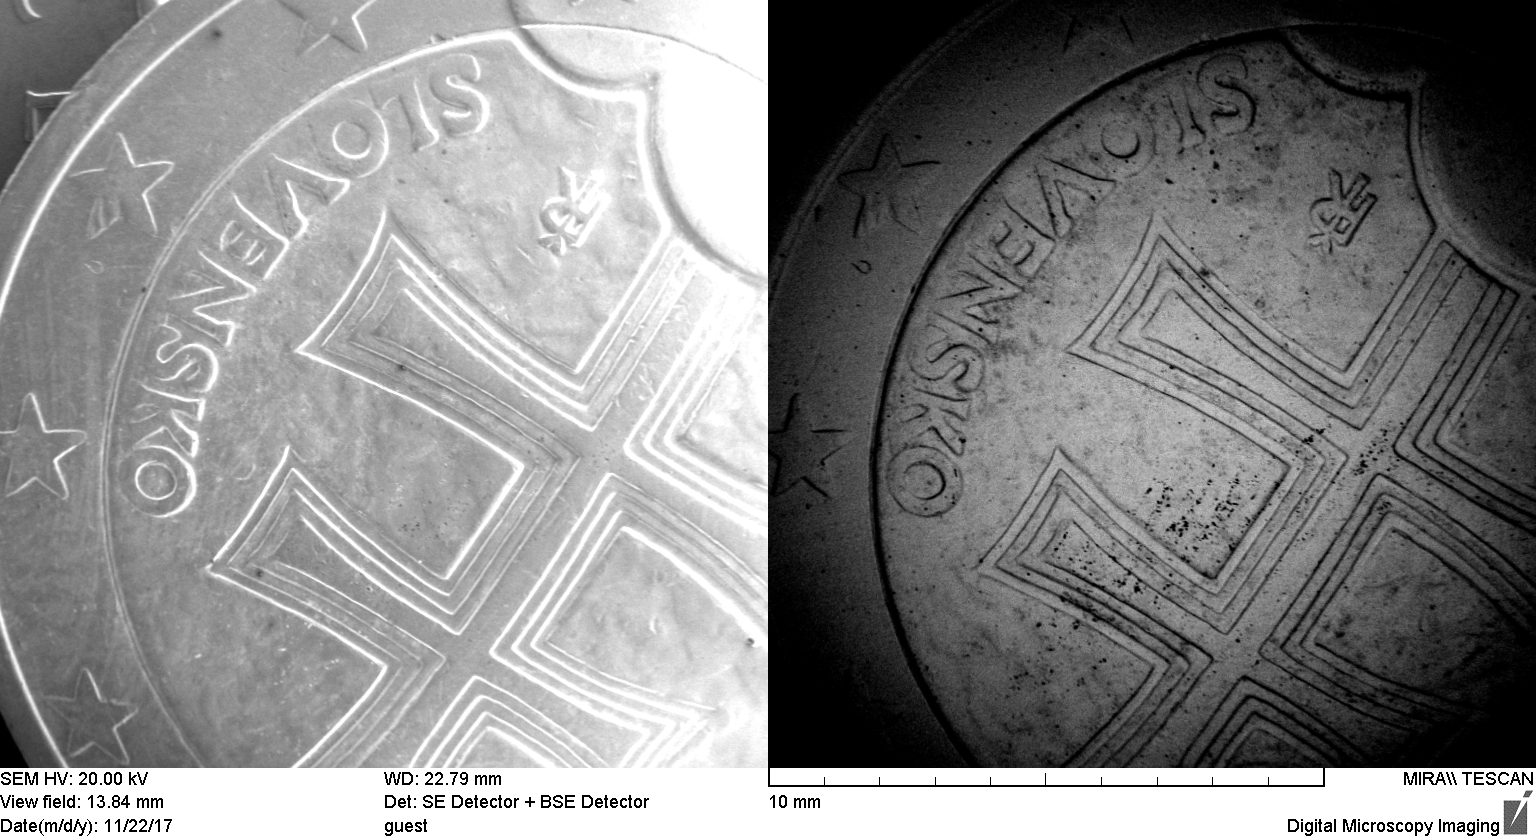
\includegraphics[width=\textwidth-2cm]{graficos/VZ01_01.png}
\caption{Vzorek 1}
\label{o:vz1_01}
\end{figure}
\begin{figure}[htbp]
\centering
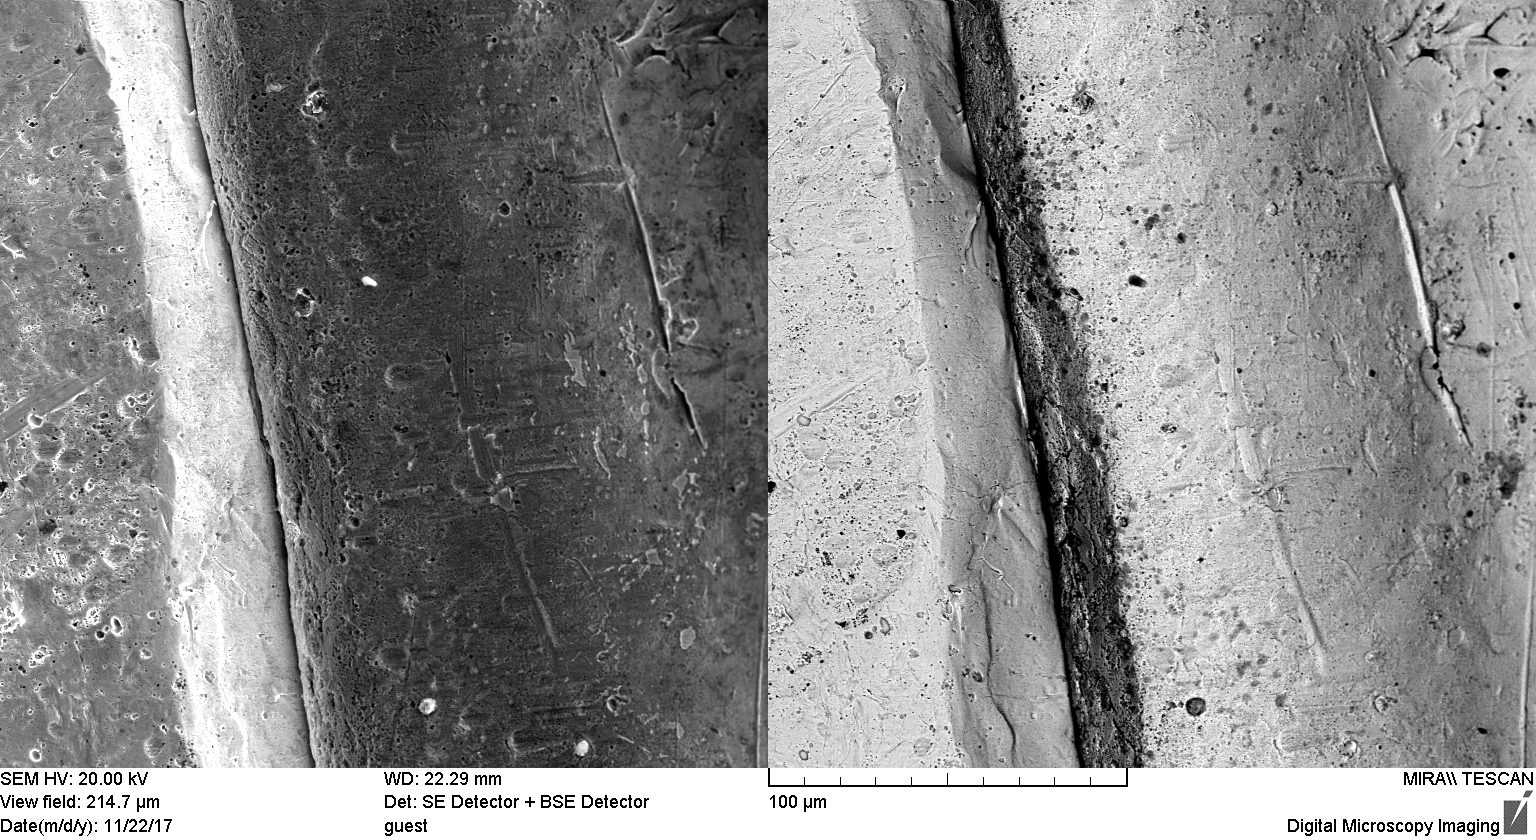
\includegraphics[width=\textwidth-2cm]{graficos/vz01_5.png}
\caption{Vzorek 1}
\label{o:vz1_05}
\end{figure}




U vzorku 2 (viz obrázek \ref{o:vz2_01}) pozorujeme kompoziční kontrast, zřejmě se skládá ze dvou fází. 
Vybrali jsme dvě místa na vzorku, bod A ve světlé oblasti BSE snímku a bod B v tmavé. 
V obou místech jsme provedli kvantitaviní analýzu RTG spektra a určili chemické složení (viz tabulky \ref{t:vz02_a} a \ref{t:vz02_b} a obrázky \ref{o:vz2_a} a \ref{o:vz2_b}). V bodě A je narozdíl od bodu B kromě hliníku přítomna těžší měď, což odpovídá tomu, že těžší prvky mají vyšší intenzitu zpětně odražených elektronů.
Dále jsme provedli lineární sken, který zde neuvádíme, a 2D sken (obrázek \ref{o:vz2_2D}).

\begin{figure}[htbp]
\centering
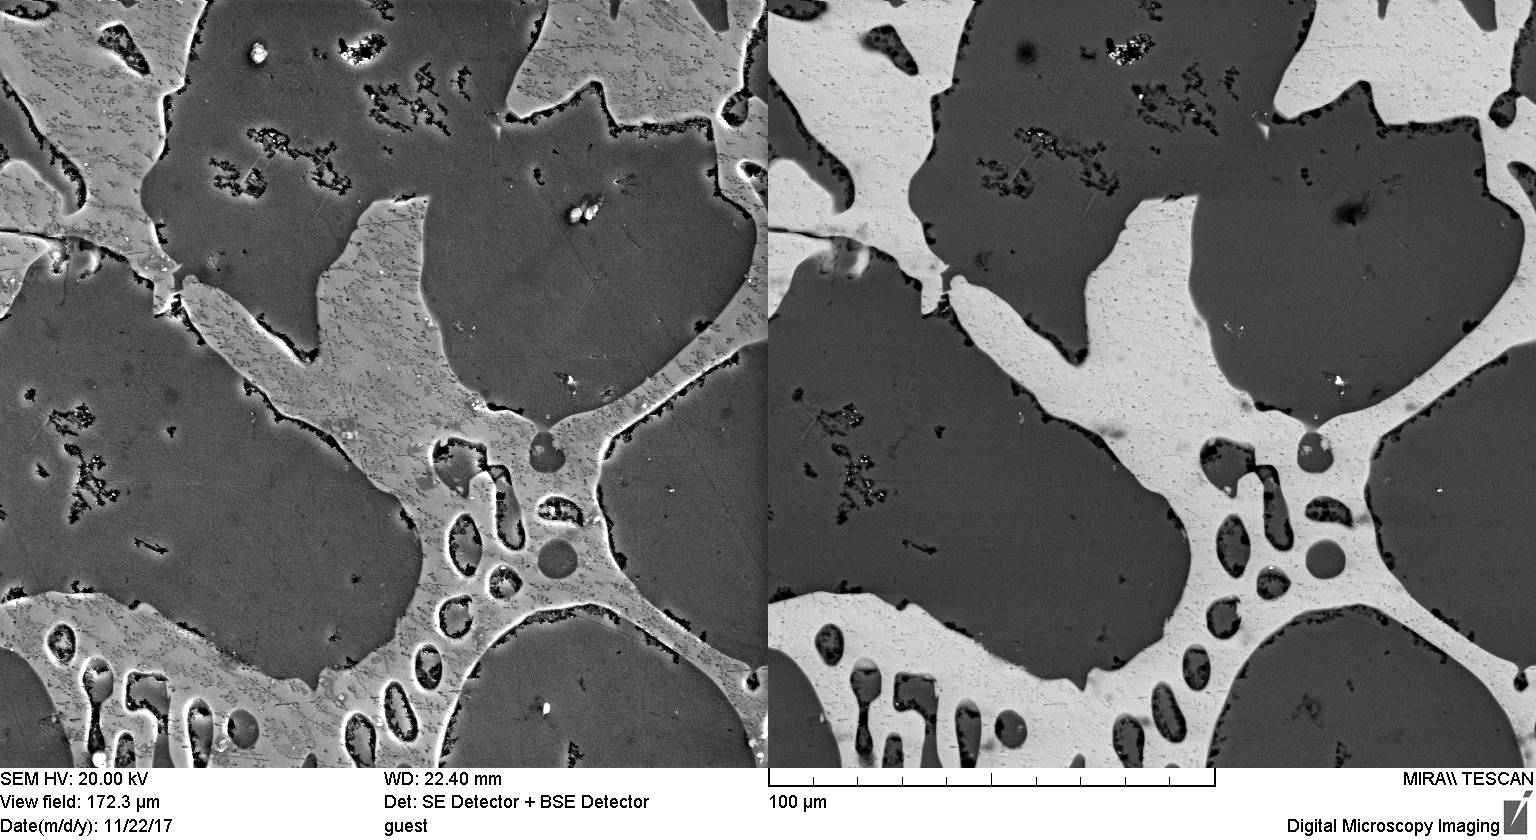
\includegraphics[width=\textwidth-2cm]{graficos/Vz02_01.png}
\caption{Vzorek 2}
\label{o:vz2_01}
\end{figure}

\begin{tabulka}[htbp]
\centering
\begin{BVerbatim}
Spectrum: Ti_Gl_1 13

Element    Series   unn. C norm. C Atom. C Error
                   [wt.-%] [wt.-%] [at.-%]   [%]
------------------------------------------------
Aluminium K-series   46,62   47,37   67,95   2,3
Copper    K-series   51,80   52,63   32,05   1,4
------------------------------------------------
            Total:   98,42  100,00  100,00
\end{BVerbatim}
\caption{Chemické složení vzorku 2 v místě A}
\label{t:vz02_a}
\end{tabulka}

\begin{figure}[htbp]
\centering
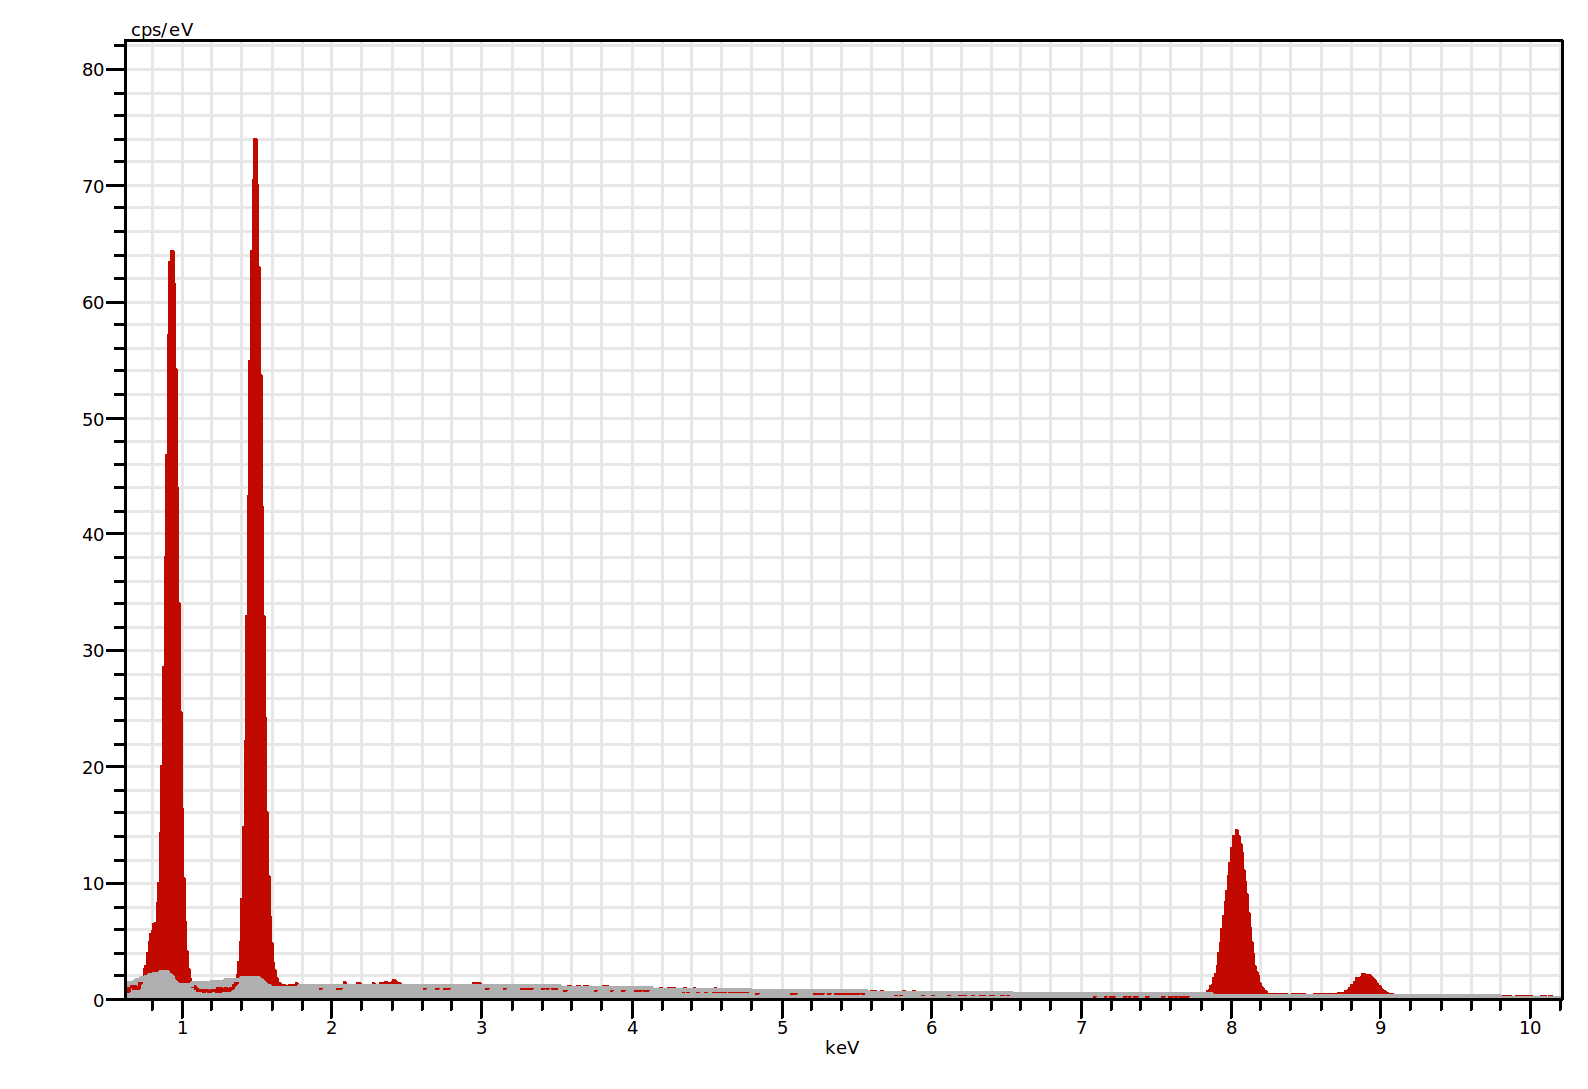
\includegraphics[width=12cm]{graficos/vz2_a.png}
\caption{Spektrum vzorku 2 v místě A}
\label{o:vz2_a}
\end{figure}

\begin{tabulka}[htbp]
\centering
\begin{BVerbatim}
Spectrum: Ti_Gl_1 14

Element    Series   unn. C norm. C Atom. C Error
                   [wt.-%] [wt.-%] [at.-%]   [%]
------------------------------------------------
Copper    K-series    5,30    4,99    2,18   0,2
Aluminium K-series  101,04   95,01   97,82   4,8
------------------------------------------------
            Total:  106,34  100,00  100,00
\end{BVerbatim}
\caption{Chemické složení vzorku 2 v místě B}
\label{t:vz02_b}
\end{tabulka}

\begin{figure}[htbp]
\centering
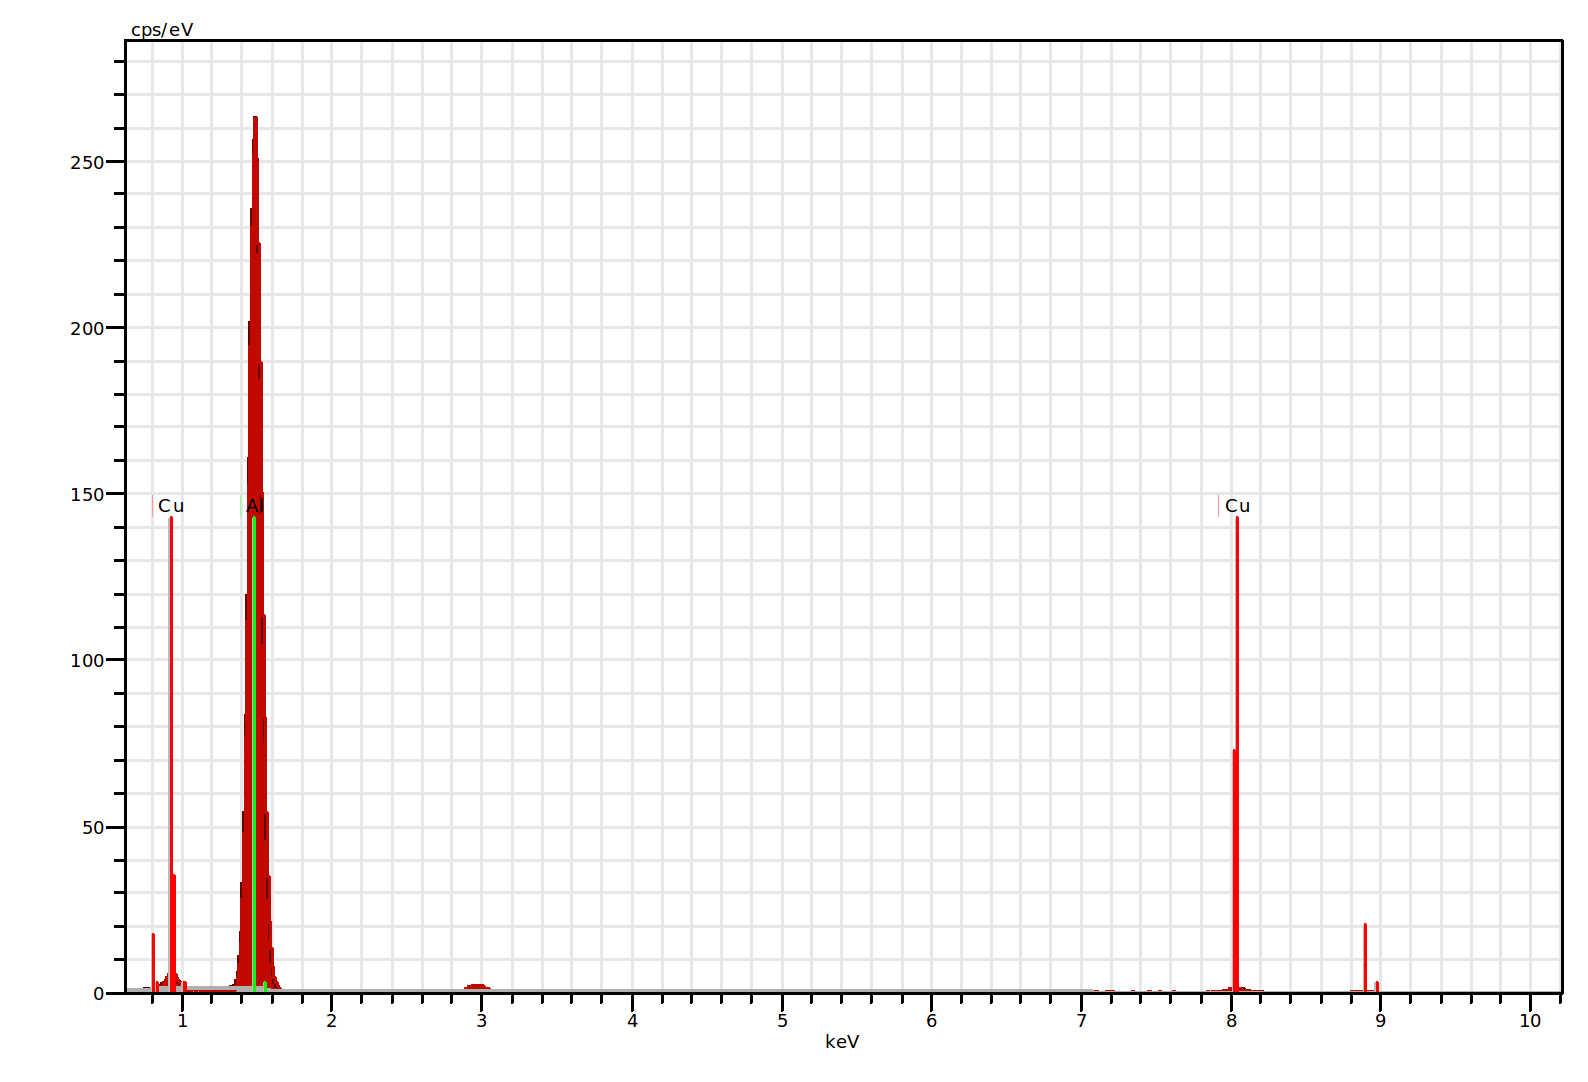
\includegraphics[width=12cm]{graficos/vz2_b.png}
\caption{Spektrum vzorku 2 v místě B}
\label{o:vz2_b}
\end{figure}

\begin{figure}[htbp]
\centering
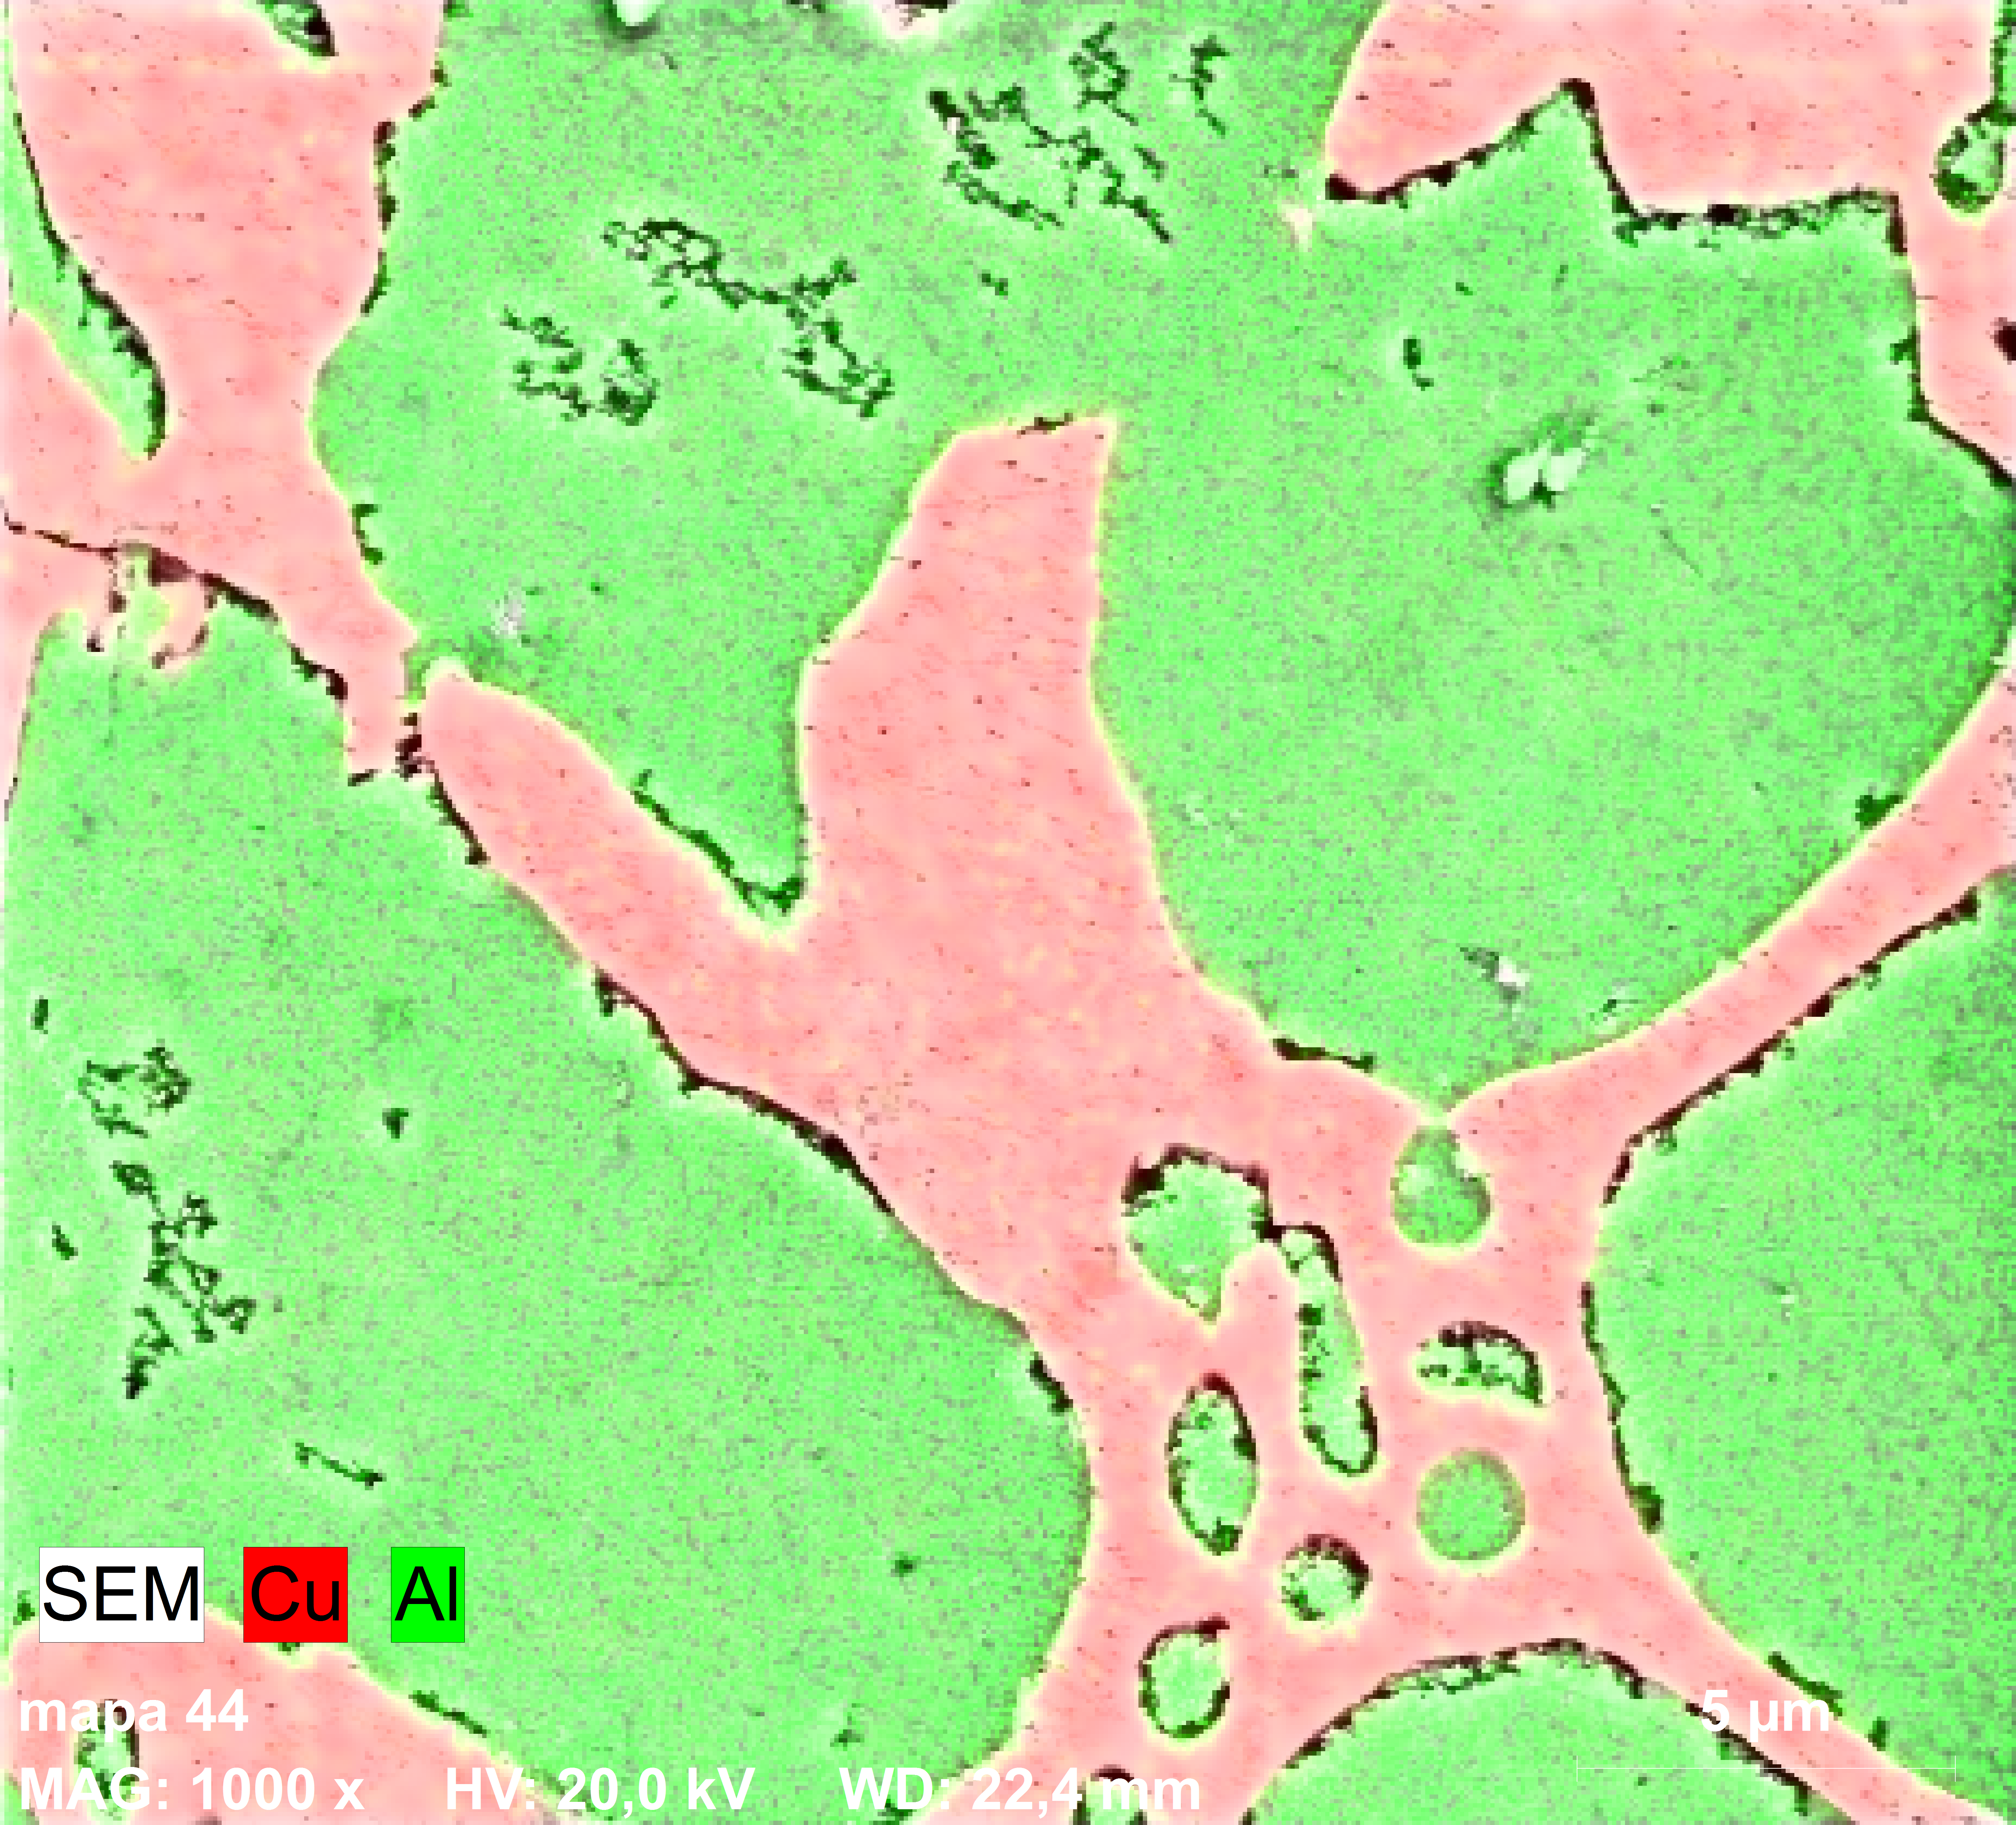
\includegraphics[width=8cm]{graficos/vz2_2D.png}
\caption{2D sken vzorku 2}
\label{o:vz2_2D}
\end{figure}
